\section{Классификация структур низкой поверхностной яркости}
В процессе визуального анализа суммарных и цветных RGB изображений было отобрано 43 галактики, имеющие приливные структуры низкой поверхностной яркости. Для более точного определения структур также использовались изображения из обзоров DESI Legacy Imaging Survey\cite{2019AJ....157..168D}, Hyper Suprime-Cam Subaru Strategic Program\cite{2022PASJ...74..247A}. 
Наблюдаемые структуры:
\begin{enumerate}
    \item Приливные хвосты -- протяженные структуры, состоящие из звезд и газа, часто образующиеся в результате крупных слияний галактик. (Рис. \ref{fig:tails})
    \item Диффузные оболочки. Под ними подразумеваем слабые протяженные гало вокруг дисков галактик, состоящие из старых звезд. Оболочки также могут являться признаком малых слияний в прошлом.(Рис. \ref{fig:shells})
    \item Мосты -- еще один подвид протяженных вытянутых структур, состоящих из звезд и газа, по сути, представляющие собой перетекание вещества от одного объекта к другому. (Рис. \ref{fig:bridges})
    \item Арки -- структуры вокруг галактики, имеющие аркообразную форму.(Рис.  \ref{fig:arcs})
    \item Остатки спутников, деформированные в процессе малого слияния. (Рис. \ref{fig:debris})
\end{enumerate}
Приливные структуры не ограничиваются списком перечисленных выше. Данные LSB структуры являются наиболее часто встречающимися в рамках нашего исследования (подробнее ознакомиться с темой галактик с приливными структурами можно, например в работе \citep{2019MNRAS.483.1470R}). Параметры галактик, обладающих приливными структурами, приведены в таблице \ref{tab:tab1}.
\begin{longtable}{|l|l|l|l|l|l|l|}
\caption{Параметры галактик из каталога ES82 обладающих приливными структурами низкой поверхностной яркости: прямое восхождение, склонение, позиционный угол, размер большой полуоси, размер малой полуоси, тип структур в соответсвии с классификацией  классификации структур, приведенной в одноименной главе (1 - приливные хвосты, 2 - диффузные оболочки, 3 - мосты, 4 - арки, 5 - полярные кольца, 6 - остатки спутников)} \label{tab:tab1}  \\ \hline
N & RA & DEC & PA  & SMA  & SMB  & structures \\ 
 &($\degree$) & ($\degree$) & ($\degree$) & (arcsec) & (arcsec) & \\ \hline\hline
        1 & 2.265 & -0.583 & -32.2 & 10 & 5.3 & 1 \\ 
        2 & 2.351 & 0.538 & 173.5 & 12.1 & 2.5 & 4 \\ 
        3 & 4.682 & -0.751 & -5.1 & 16.8 & 7.9 & 4 \\ 
        4 & 7.35 & 0.316 & 22.6 & 32 & 8.1 & 4 \\ 
        5 & 13.728 & 0.434 & 77.9 & 13.8 & 3.6 & 3 \\ 
        6 & 14.094 & -0.345 & 4.7 & 17.5 & 8.2 & 3, 4 \\ 
        7 & 14.463 & -0.418 & 82.4 & 10 & 5.2 & 4 \\ 
        8 & 15.846 & -0.469 & -75.9 & 11.2 & 5.5 & 1 \\ 
        9 & 17.089 & 0.044 & -24.8 & 10.5 & 4.5 & 1 \\ 
        10 & 17.898 & 0.462 & 88.29 & 26.5 & 6.6 & 4 \\ 
        11 & 19.434 & 0.254 & -64.7 & 22.3 & 12.1 & 2 \\ 
        12 & 20.13 & 0.786 & -28.7 & 10.9 & 4.3 & 3 \\ 
        13 & 20.271 & 0.103 & 33 & 19.7 & 4.4 & 2 4 \\ 
        14 & 20.523 & 0.085 & -47.09 & 44.6 & 6.1 & 2, 4 \\ 
        15 & 21.171 & 0.081 & -50.58 & 24.1 & 5.9 & 4 \\ 
        16 & 23.504 & -0.537 & -73.8 & 10.3 & 4.5 & 2 \\ 
        17 & 24.765 & 0.437 & -20.7 & 21.8 & 7.3 & 2 \\ 
        18 & 28.031 & -0.126 & 13.6 & 8.5 & 6.2 & 1 \\ 
        19 & 28.265 & 1.023 & 74.99 & 16.3 & 4.8 & 4 \\ 
        20 & 30.191 & -0.908 & 57.3 & 27.3 & 8.7 & 4 \\ 
        21 & 31.972 & -0.028 & -66.6 & 8.1 & 4.1 & 1, 3, 4 \\ 
        22 & 32.794 & -0.517 & -52.2 & 18.2 & 4.4 & 1 \\ 
        23 & 37.653 & -0.824 & -78.6 & 10.1 & 5.4 & 3 \\ 
        24 & 37.936 & -0.945 & -48.6 & 19.2 & 9.9 & 4 \\ 
        25 & 38.657 & -0.98 & -36.15 & 43.5 & 10.5 & 4 \\ 
        26 & 46.894 & -1.049 & -21.9 & 22.8 & 10.4 & 4 \\ 
        27 & 47.102 & -0.559 & 14 & 34 & 6.3 & 2 \\ 
        28 & 49.36 & -0.094 & 116.99 & 44.3 & 11.9 & 2 \\ 
        29 & 52.605 & 0.274 & -80.4 & 20.9 & 10.1 & 4 \\ 
        30 & 311.043 & -0.415 & 326.99 & 16.1 & 3.3 & 2 \\ 
        31 & 314.206 & -0.238 & -5.2 & 15.8 & 4.5 & 4 \\ 
        32 & 315.137 & 0.294 & 16.4 & 30.3 & 8.3 & 4 \\ 
        33 & 316.508 & -0.504 & 36.9 & 8.4 & 3.1 & 4 \\ 
        34 & 323.964 & -0.278 & 15.43 & 11.9 & 5.7 & 1 \\ 
        35 & 325.543 & -0.288 & 50.31 & 8.2 & 6.7 & 2, 4 \\ 
        36 & 336.825 & -0.682 & -6.3 & 12.9 & 4.4 & 4 \\ 
        37 & 337.223 & 0.771 & -27.3 & 16.2 & 9.1 & 4 \\ 
        38 & 340.706 & -0.607 & -41.6 & 9.7 & 5.9 & 4 \\ 
        39 & 343.094 & 1.093 & 99.9 & 78.5 & 46.1 & 2 \\ 
        40 & 344.174 & 0.162 & 9.2 & 18.9 & 5.4 & 2 \\ 
        41 & 350.214 & -1.011 & -31.5 & 15.2 & 7.4 & 2 \\ 
        42 & 350.832 & -0.5 & -5.63 & 13 & 4 & 1, 4 \\ 
        43 & 353.011 & 1.223 & 13.5 & 16.7 & 6.1 & 2 \\ 
        44 & 353.902 & -0.976 & 103.3 & 15.1 & 4.9 & 4 \\\hline

\end{longtable}

Помимо приливных структур, были выделены еще некоторые структурные особенности галактик -- 86 объектов, см таблицу ~\ref{tab:tab2}(подробнее про структурные особенности галактик можно найти, например, в  \citep{van_der_Kruit_2011}, \citep{2020MNRAS.497.2039M}):
\begin{enumerate}
    \item Толстые коробкоподобные балджи (Рис. \ref{fig:bulge})
    \item Полярные балджи (Рис. \ref{fig:bulge})
    \item Кособокость (lopsidedness -- смещение центральной части галактики) (Рис. \ref{fig:lopsided})
    \item Изгибы звездного диска (Рис. \ref{fig:warp})
    \item Полярные кольца -- структуры, состоящие из звезд и газа, в большинстве случаев ориентированные перпендикулярно к плоскости звездного диска галактики. (Рис. \ref{fig:rings}) 
\end{enumerate}

\begin{longtable}{|l|l|l|l|l|l|l|}
\caption{Параметры галактик из каталога ES82 обладающих структурными особенностями: прямое восхождение, склонение, позиционный угол, размер большой полуоси, размер малой полуоси, типы структур в соответствии с классификацией, приведенной в одноименной главе (1 - коробкоподобные балджи, 2 - полярные балджи, 3 - кособокость, 4 - изгиб звездного диска, 5 - спирали).} \label{tab:tab2} \\\hline
    
 N & RA & DEC & PA  & SMA  & SMB  & structures \\ 
 &($\degree$) & ($\degree$) & ($\degree$) & (arcsec) & (arcsec) & \\
 \hline \hline 
        1 & 331.378 & 0.077 & 25.59 & 34.1 & 7.4 & 1,4 \\ 
        2 & 346.594 & -0.822 & 30.26 & 18.3 & 2.9 & 4 \\ 
        3 & 347.324 & 0.064 & -55.3 & 35.1 & 8.9 & 2, 4 \\ 
        4 & 349.019 & -0.123 & 7.99 & 24 & 5.9 & 4 \\ 
        5 & 350.832 & -0.5 & -5.63 & 13 & 4 & 4 \\ 
        6 & 10.652 & 0.831 & -88.01 & 7.9 & 2.3 & 1 \\ 
        7 & 17.898 & 0.462 & 88.29 & 26.5 & 6.6 & 4 \\ 
        8 & 18.239 & -0.345 & -73.6 & 55.4 & 11.9 & 4 \\ 
        9 & 21.171 & 0.081 & -50.58 & 24.1 & 5.9 & 4 \\ 
        10 & 25.149 & 0.259 & 45.96 & 20.7 & 5.9 & 3 \\ 
        11 & 32.777 & -0.655 & 17.38 & 24.4 & 4.8 & 3, 4 \\ 
        12 & 37.911 & -1.083 & 84.17 & 24 & 6.6 & 4 \\ 
        13 & 0.418 & 1.092 & 18.6 & 35.9 & 9.5 & 1 \\ 
        14 & 0.836 & -0.527 & -8 & 10 & 6.1 & 1 \\ 
        15 & 1.135 & 0.909 & 0.4 & 12.8 & 5.1 & 2 \\ 
        16 & 1.87 & 0.902 & 24 & 17.9 & 6.2 & 3 \\ 
        17 & 3.013 & -1.007 & -72.8 & 12.1 & 6 & 2 \\ 
        18 & 4.917 & 0.867 & -51 & 18.7 & 6.1 & 2 \\ 
        19 & 5.541 & -0.937 & 70.1 & 16.8 & 8.2 & 1 \\ 
        20 & 5.583 & 0.009 & 172.1 & 33.9 & 7.1 & 4 \\ 
        21 & 5.724 & -0.997 & -53 & 14.8 & 7.9 & 1, 3, 4 \\ 
        22 & 5.982 & -1.146 & -79.4 & 12.8 & 6.7 & 1 \\ 
        23 & 6.036 & 0.379 & 61.3 & 15.7 & 4.3 & 3 \\ 
        24 & 7.421 & 0.563 & -71.5 & 15.3 & 3.7 & 4 \\ 
        25 & 7.628 & -0.781 & 70.6 & 26.8 & 7 & 5 \\ 
        26 & 8.41 & -0.812 & -75.7 & 14.2 & 5.2 & 2 \\ 
        27 & 10.574 & 0.371 & 63.16 & 24.2 & 7.7 & 4 \\ 
        28 & 13.396 & 0.596 & -43.9 & 16.5 & 7.3 & 4 \\ 
        29 & 13.728 & 0.434 & 77.9 & 13.8 & 3.6 & 4 \\ 
        30 & 14.082 & -0.126 & 165.9 & 25.5 & 6.4 & 4 \\ 
        31 & 14.789 & 0.198 & 26.8 & 10.4 & 4.3 & 1 \\ 
        32 & 16.599 & -0.17 & 43.1 & 12.1 & 8.5 & 2, 4 \\ 
        33 & 17.693 & 0.793 & 9.7 & 13.3 & 4.8 & 4 \\ 
        34 & 18.239 & -0.345 & 18.6 & 38.4 & 9 & 4 \\ 
        35 & 19.468 & 0.781 & 3.7 & 21.9 & 7.6 & 4, 5 \\ 
        36 & 20.482 & 0.066 & -64.1 & 22.4 & 5.9 & 2 \\ 
        37 & 20.532 & 0.811 & 17.3 & 12 & 6.1 & 2 \\ 
        38 & 21.159 & -0.063 & -36 & 37.9 & 11.8 & 2 \\ 
        39 & 22.535 & 0.565 & -5.7 & 8.9 & 4.3 & 2 \\ 
        40 & 22.977 & 0.492 & 15.5 & 24.5 & 5.7 & 4 \\ 
        41 & 23.504 & -0.537 & -73.8 & 10.3 & 4.5 & 2 \\ 
        42 & 23.639 & -0.43 & 40.4 & 15.8 & 7.2 & 2, 4 \\ 
        43 & 23.752 & -0.451 & 14.7 & 24.1 & 7.8 & 4 \\ 
        44 & 24.493 & -0.889 & -67 & 18.8 & 5.2 & 2 \\ 
        45 & 27.115 & 0.394 & 2 & 10.4 & 5.8 & 2, 4 \\ 
        46 & 27.561 & 0.062 & 21.6 & 12 & 4.2 & 4 \\ 
        47 & 29.228 & -1.115 & 63.1 & 27.7 & 13.4 & 1 \\ 
        48 & 29.237 & 1.168 & 54.4 & 18.8 & 4.9 & 4 \\ 
        49 & 29.471 & -1.167 & 12.4 & 11.1 & 6.5 & 2 \\ 
        50 & 30.181 & 1.019 & 15.7 & 19.2 & 5.2 & 2, 4 \\ 
        51 & 30.569 & -0.533 & 64.4 & 28.3 & 5.1 & 4 \\ 
        52 & 31.245 & -0.264 & 89 & 22.3 & 4.7 & 4 \\ 
        53 & 31.595 & 0.907 & -9.8 & 12.9 & 5.7 & 2 \\ 
        54 & 32.676 & -0.638 & 17.4 & 23.2 & 8.2 & 2 \\ 
        55 & 32.722 & -0.921 & 2.44 & 25.3 & 4.2 & 2, 4 \\ 
        56 & 33.789 & -0.704 & -26 & 24.3 & 5 & 2 \\ 
        57 & 39.177 & -0.017 & 70.1 & 26.7 & 7 & 4 \\ 
        58 & 41.525 & 0.564 & 41.7 & 22.1 & 6.6 & 4 \\ 
        59 & 42.143 & -0.993 & -1.5 & 44.2 & 14.2 & 1, 4 \\ 
        60 & 49.642 & -0.362 & 25.6 & 22 & 5.1 & 4 \\ 
        61 & 56.608 & -0.599 & -14.7 & 25.3 & 6.8 & 4 \\ 
        62 & 313.353 & 0.652 & 17.69 & 53.8 & 11.4 & 4 \\ 
        63 & 314.393 & 0.341 & -84.1 & 43.6 & 9.5 & 4 \\ 
        64 & 315.137 & 0.294 & 16.4 & 30.3 & 8.3 & 4, 5 \\ 
        65 & 326.305 & -0.186 & -84.68 & 17.5 & 4.6 & 4 \\ 
        66 & 319.276 & -0.627 & 76 & 17.8 & 4.5 & 3 \\ 
        67 & 320.078 & -1.093 & 81.5 & 18.6 & 5.1 & 3 \\ 
        68 & 328.247 & 0.567 & 37.4 & 16.7 & 6 & 3 \\ 
        69 & 333.752 & 0.804 & 51.5 & 25.7 & 6.1 & 3 \\ 
        70 & 336.167 & -0.897 & -23.1 & 14 & 8.3 & 2, 4 \\ 
        71 & 336.384 & 0.039 & -5.7 & 12.4 & 5.1 & 4, 5 \\ 
        72 & 339.008 & -0.56 & 68.3 & 18.8 & 6.3 & 4 \\ 
        73 & 341.096 & -0.114 & -0.1 & 17.1 & 4.7 & 4 \\ 
        74 & 343.78 & -0.891 & 4.3 & 12 & 6.5 & 2 \\ 
        75 & 346.764 & 0.35 & -1.6 & 20.7 & 5.2 & 4 \\ 
        76 & 347.624 & 0.273 & 84.5 & 11 & 4.5 & 4 \\ 
        77 & 348.063 & -0.064 & -35.5 & 14 & 3.9 & 1 \\ 
        78 & 350.532 & 0.402 & 40.7 & 12.8 & 7.4 & 2 \\ 
        79 & 351.14 & -0.731 & -30.2 & 15.9 & 10.1 & 4 \\ 
        80 & 352.972 & -0.827 & 108 & 41.7 & 11.2 & 4 \\ 
        81 & 353.011 & 1.223 & 13.5 & 16.7 & 6.1 & 3 \\ 
        82 & 354.641 & 0.281 & -8.9 & 10.9 & 5.8 & 2 \\ 
        83 & 355.229 & -1.074 & 33.7 & 17.1 & 6.1 & 2, 4 \\ 
        84 & 355.724 & 0.705 & 30 & 10.4 & 4.6 & 2 \\ 
        85 & 359.526 & -0.987 & -2.4 & 14.2 & 6.2 & 2 \\ \hline 

\end{longtable}

\begin{figure}[ht]

    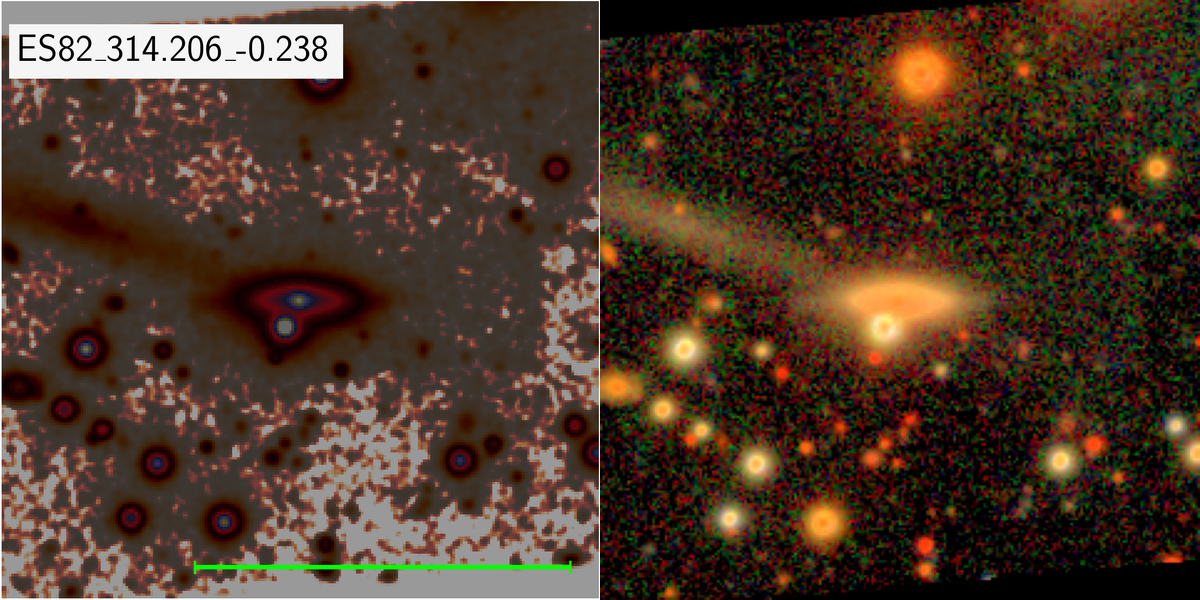
\includegraphics[width=.5\textwidth]{images/526.png}\hfill
    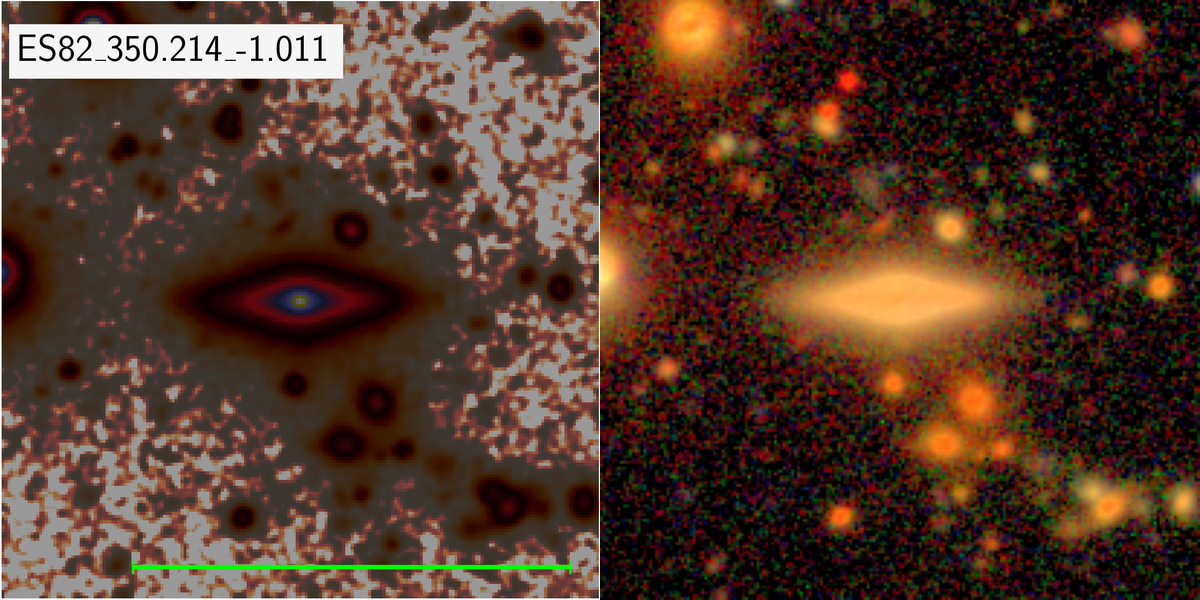
\includegraphics[width=.5\textwidth]{images/777.png}\hfill
    \caption{Примеры галактик с хвостами. Левая панель -- суммарное изображение галактики, правая панель -- цветное RGB изображение.}\label{fig:tails}
\end{figure}

\begin{figure}[ht]

    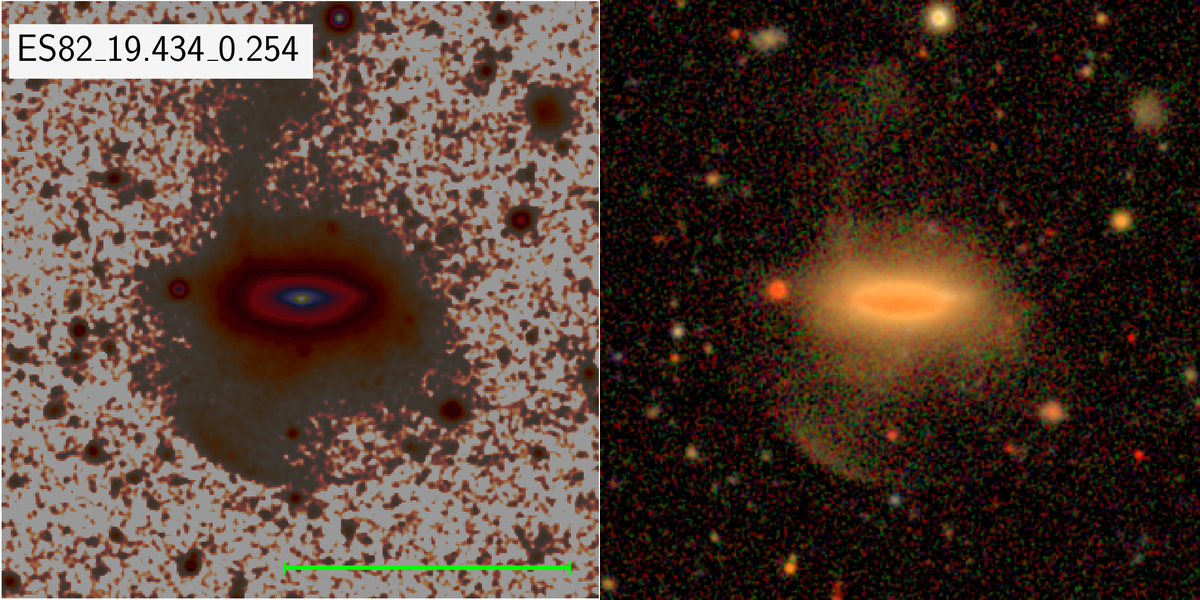
\includegraphics[width=.5\textwidth]{images/222.png}\hfill
    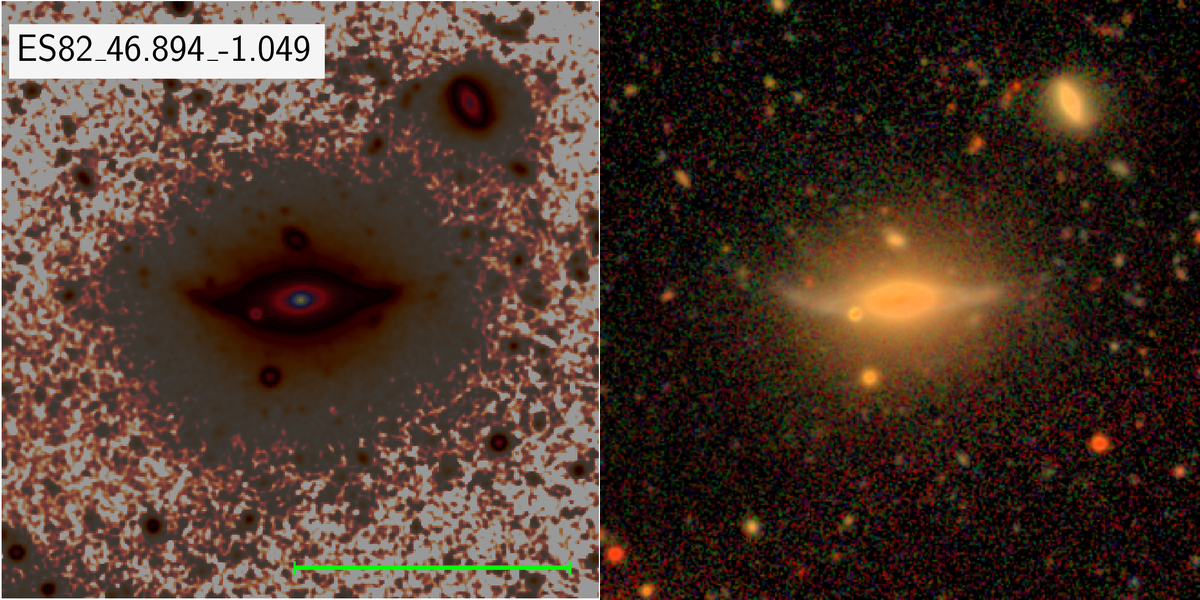
\includegraphics[width=.5\textwidth]{images/424.png}\hfill

    \caption{Примеры галактик с оболочками. Левая панель -- суммарное изображение галактики, правая панель -- цветное RGB изображение.}\label{fig:shells}
\end{figure}

\begin{figure}[ht]

    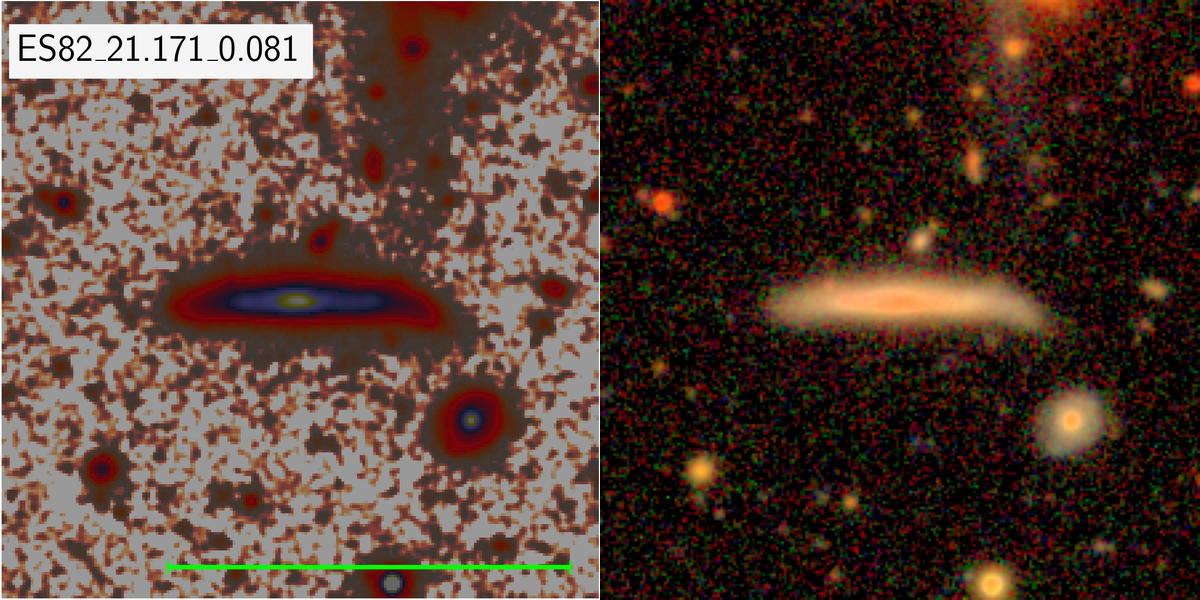
\includegraphics[width=.5\textwidth]{images/247.png}\hfill
    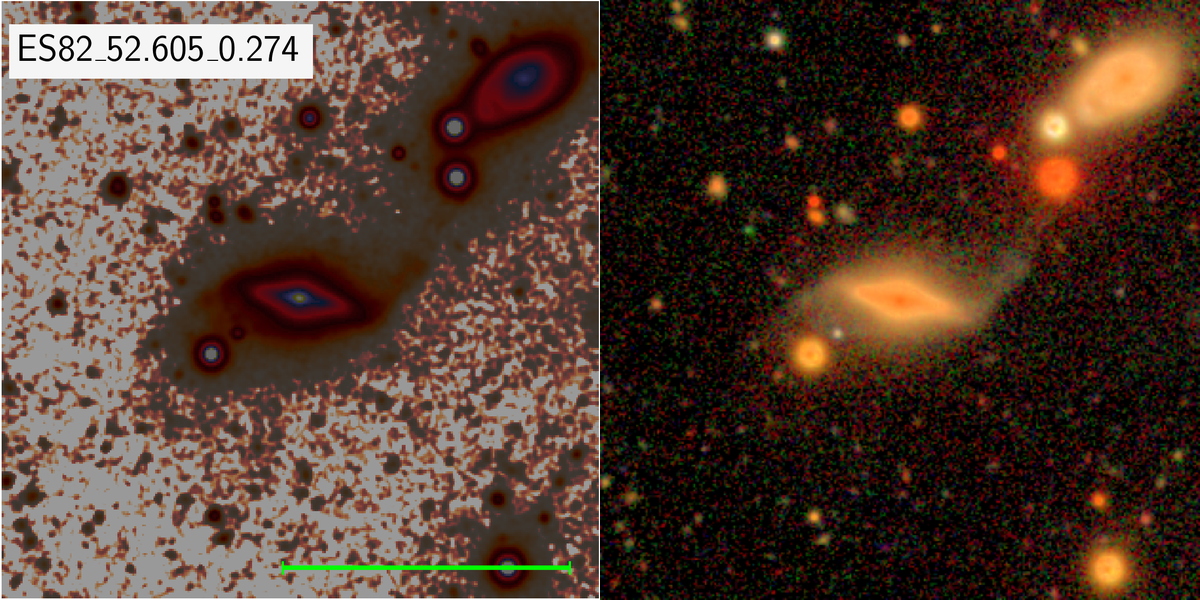
\includegraphics[width=.5\textwidth]{images/471.png}\hfill
    \caption{Примеры галактик с мостами. Левая панель -- суммарное изображение галактики, правая панель -- цветное RGB изображение.}\label{fig:bridges}
\end{figure}

\begin{figure}[ht]

    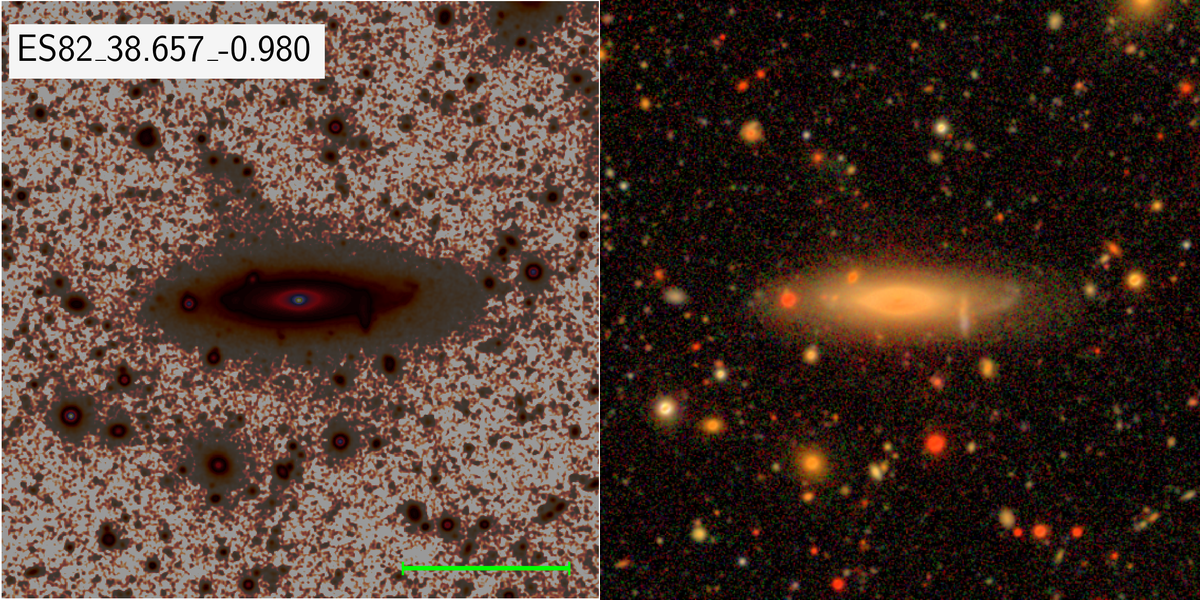
\includegraphics[width=.5\textwidth]{images/52.png}\hfill
    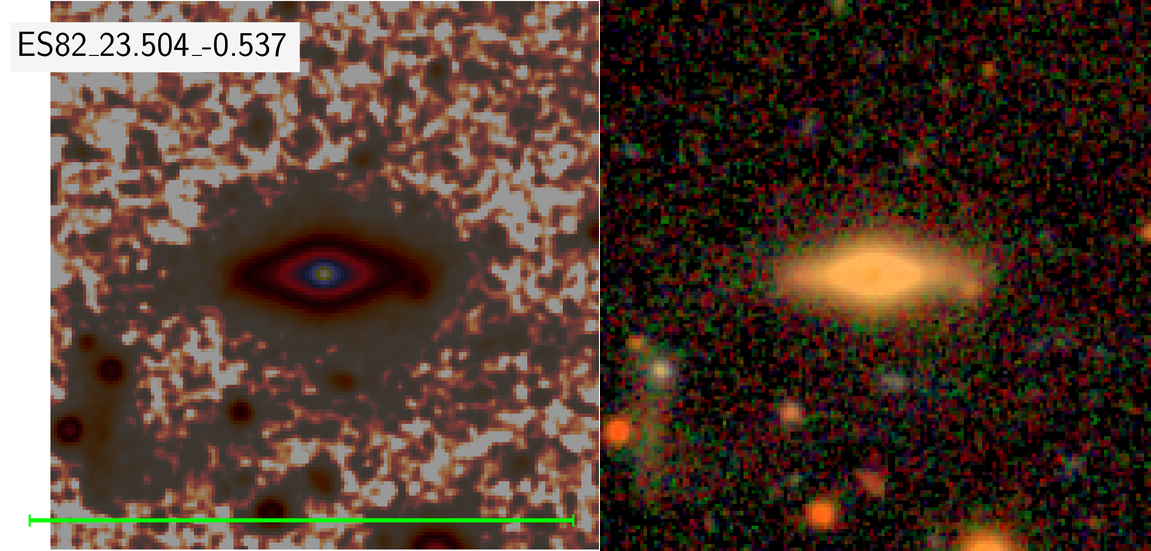
\includegraphics[width=.5\textwidth]{images/262.png}\hfill

    \caption{Примеры галактик с арками. Левая панель -- суммарное изображение галактики, правая панель -- цветное RGB изображение.}\label{fig:arcs}
\end{figure}

\begin{figure}[ht]

    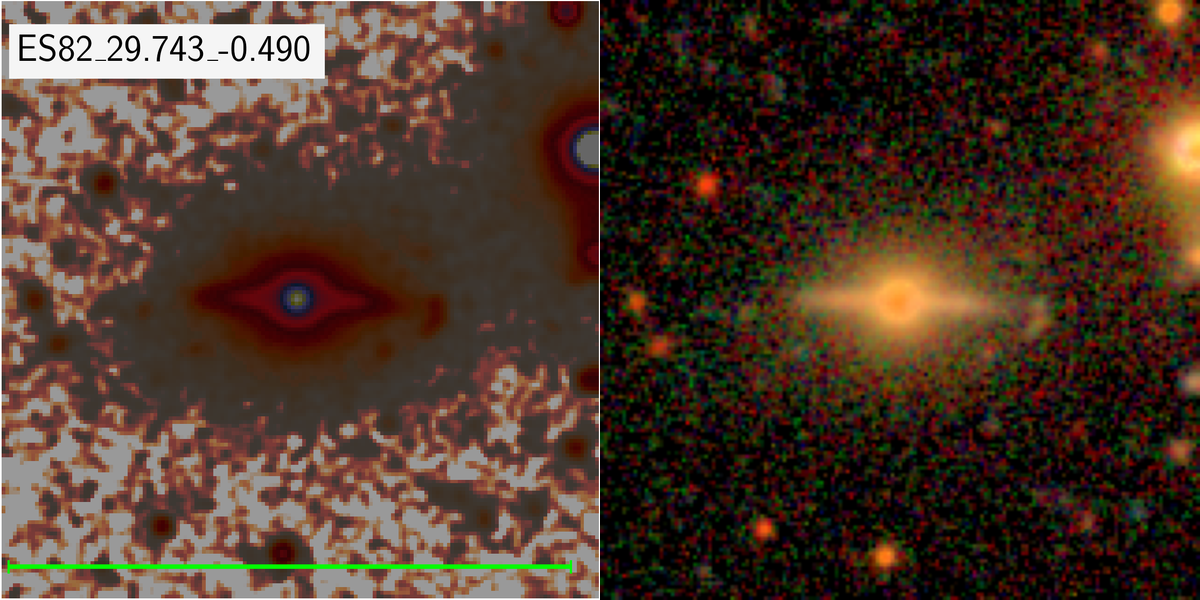
\includegraphics[height=.14\textheight]{images/307.png}\hfill
    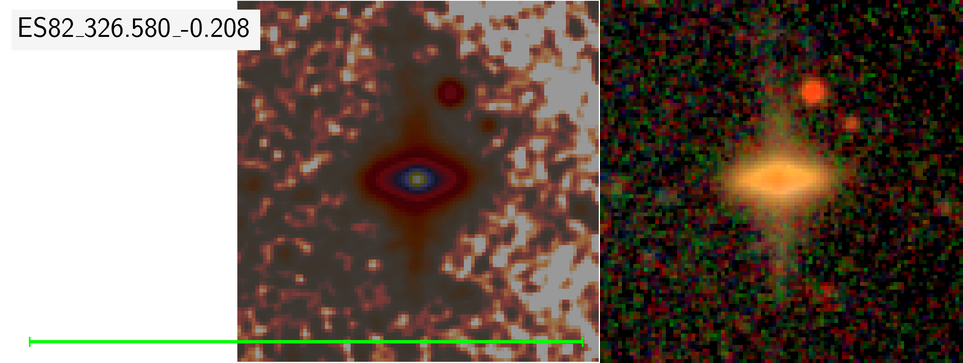
\includegraphics[height=.14\textheight]{images/627.png}\hfill

    \caption{Примеры галактик с полярными кольцами. Левая панель -- суммарное изображение галактики, правая панель -- цветное RGB изображение.}\label{fig:rings}
\end{figure}

\begin{figure}[ht]

    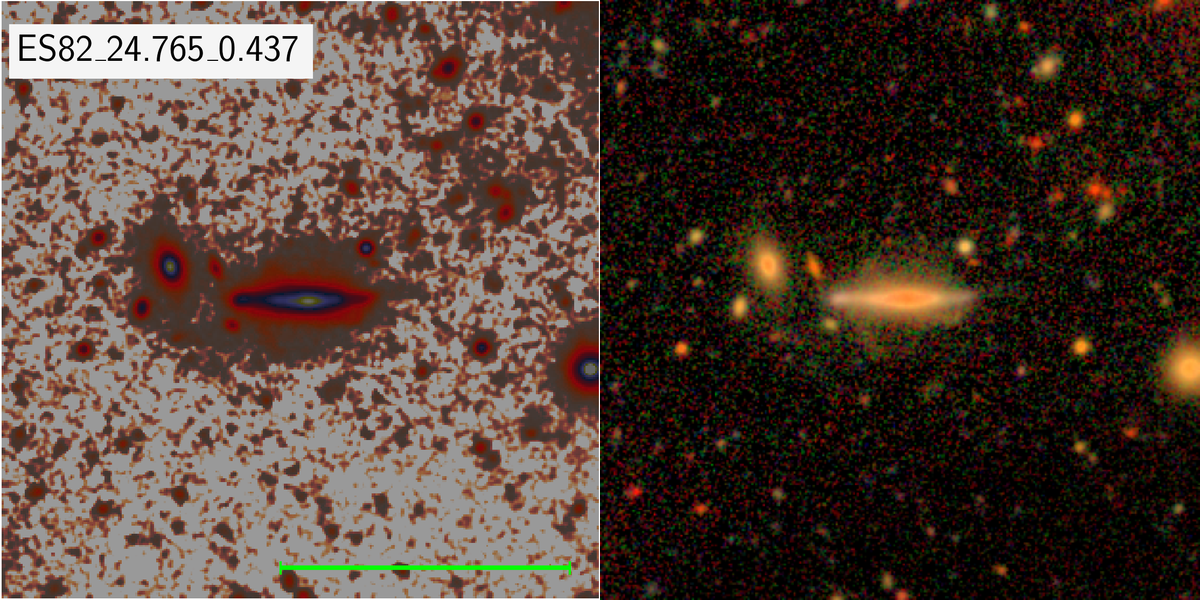
\includegraphics[width=.5\textwidth]{images/270.png}\hfill
    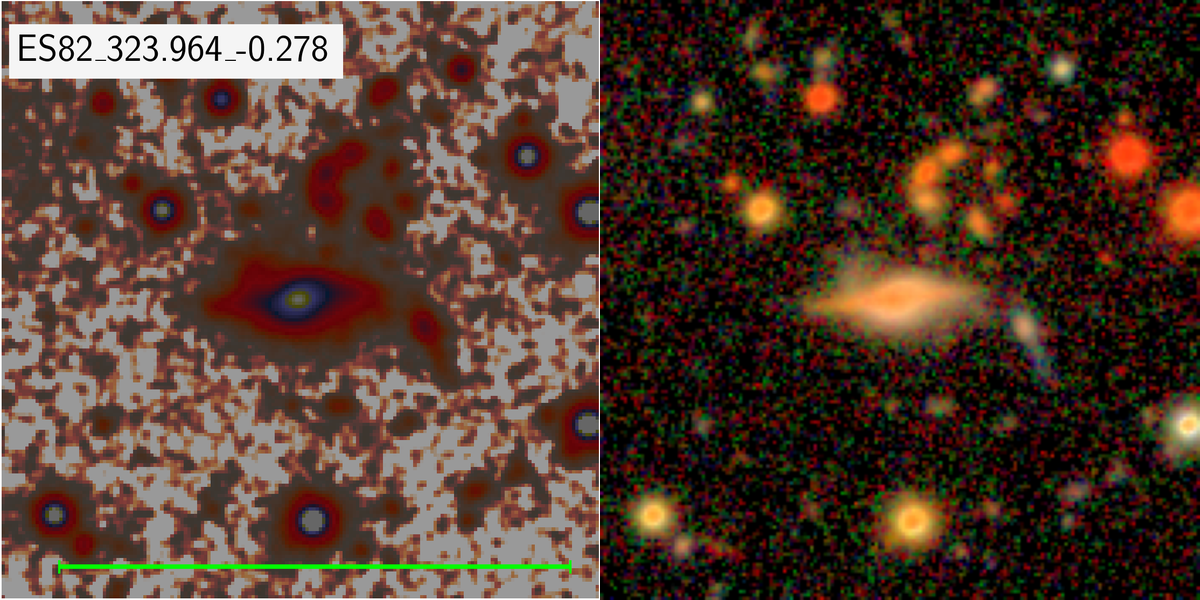
\includegraphics[width=.5\textwidth]{images/602.png}\hfill

    \caption{Примеры галактик с остатками спутников. Левая панель -- суммарное изображение галактики, правая панель -- цветное RGB изображение.}\label{fig:debris}
\end{figure}

\begin{figure}[ht]

    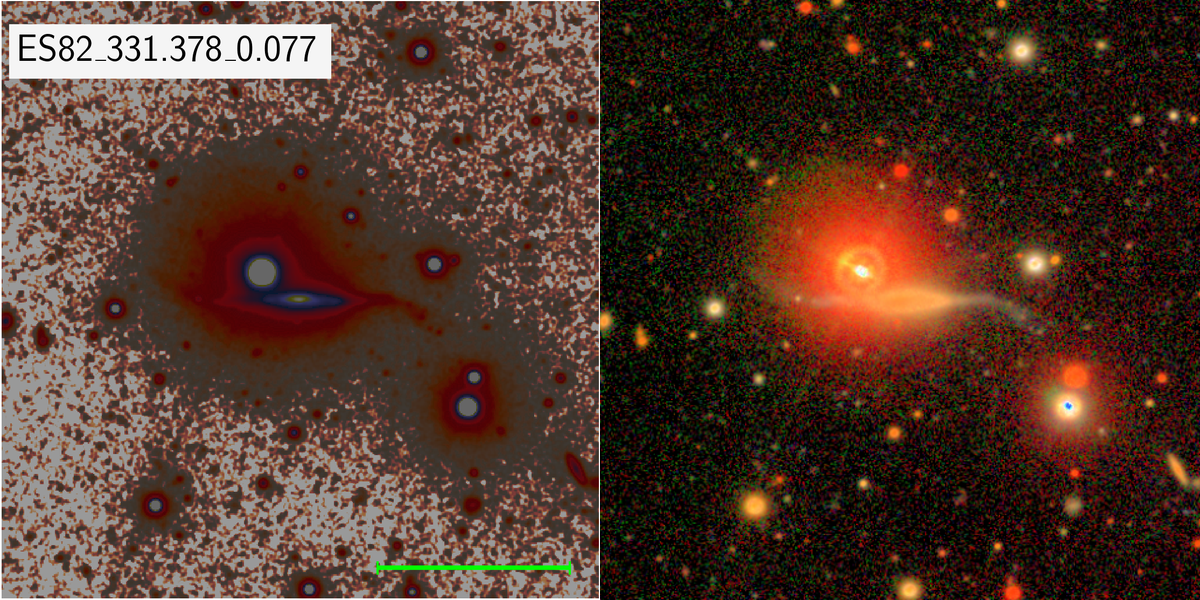
\includegraphics[width=.5\textwidth]{images/11.png}\hfill
    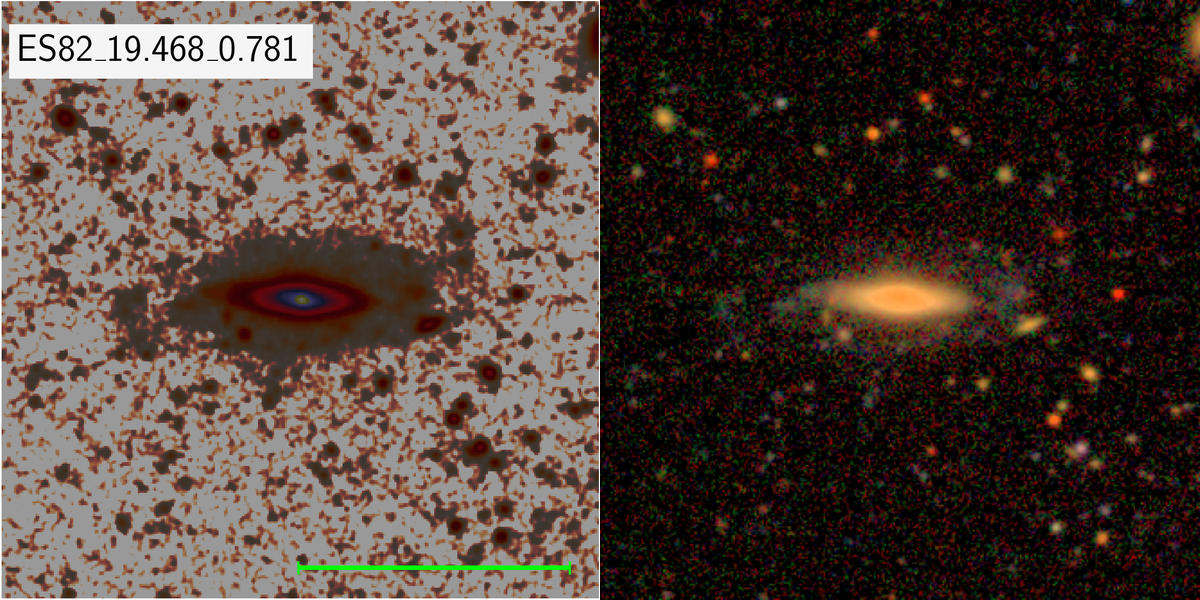
\includegraphics[width=.5\textwidth]{images/224.png}\hfill

    \caption{Примеры галактик с изгибами диска. Левая панель -- суммарное изображение галактики, правая панель -- цветное RGB изображение.}\label{fig:warp}
\end{figure}

\begin{figure}[ht]

    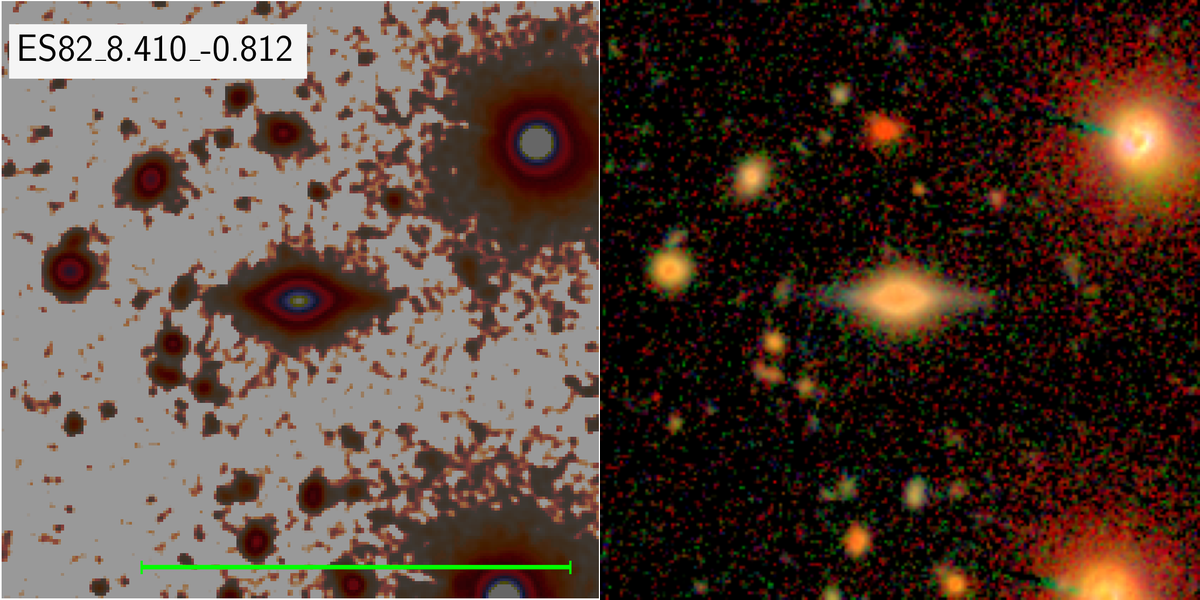
\includegraphics[width=.5\textwidth]{images/139.png}\hfill
    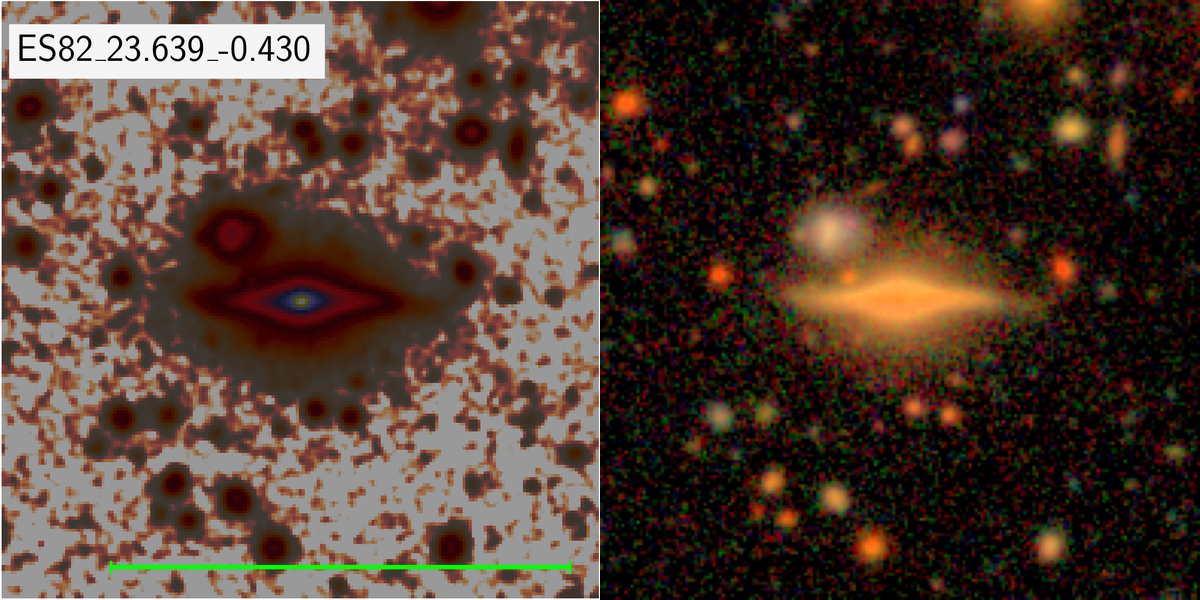
\includegraphics[width=.5\textwidth]{images/263.png}\hfill

    \caption{Примеры галактик с балджем. Левая панель -- суммарное изображение галактики, правая панель -- цветное RGB изображение.}\label{fig:bulge}
\end{figure}

\begin{figure}[ht]

    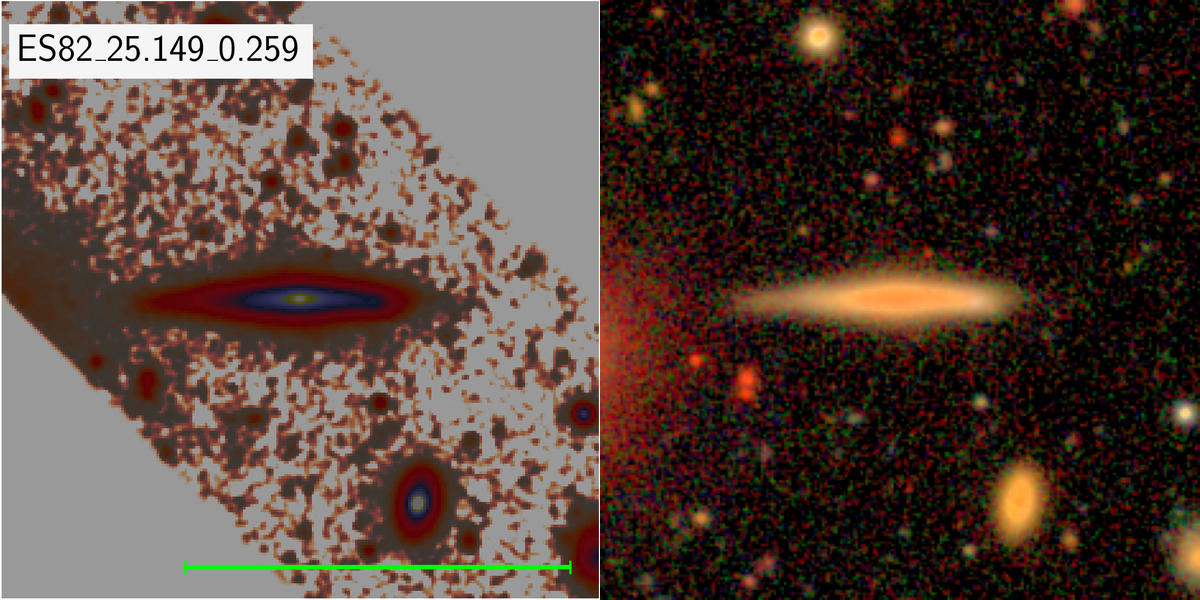
\includegraphics[width=.5\textwidth]{images/45.png}\hfill
    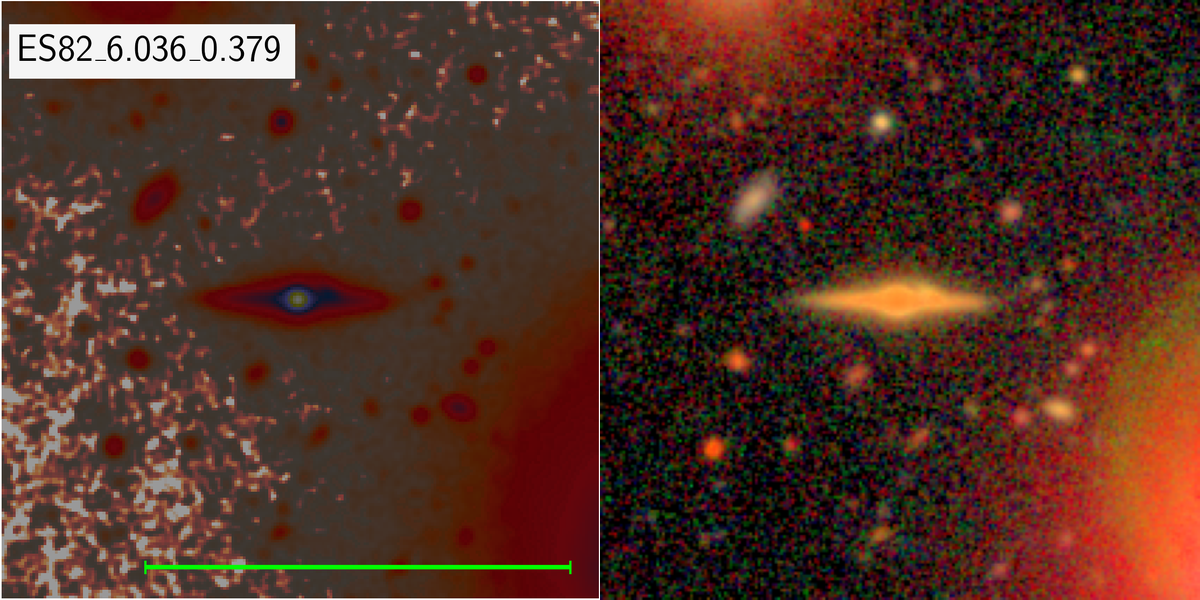
\includegraphics[width=.5\textwidth]{images/118.png}\hfill

    \caption{Примеры галактик с кособокими звездными дисками. Левая панель -- суммарное изображение галактики, правая панель -- цветное RGB изображение.}\label{fig:lopsided}
\end{figure}
